% This file was converted to LaTeX by Writer2LaTeX ver. 1.4
% see http://writer2latex.sourceforge.net for more info
\documentclass[a4paper]{article}
\usepackage[ascii]{inputenc}
\usepackage[T1]{fontenc}
\usepackage[english]{babel}
\usepackage{amsmath}
\usepackage{amssymb,amsfonts,textcomp}
\usepackage{color}
\usepackage{array}
\usepackage{supertabular}
\usepackage{hhline}
\usepackage{hyperref}
\hypersetup{pdftex, colorlinks=true, linkcolor=blue, citecolor=blue, filecolor=blue, urlcolor=blue, pdftitle=, pdfauthor=, pdfsubject=, pdfkeywords=}
\usepackage[pdftex]{graphicx}
% footnotes configuration
\makeatletter
\renewcommand\thefootnote{\arabic{footnote}}
\makeatother
% Outline numbering
\setcounter{secnumdepth}{0}
\makeatletter
\newcommand\arraybslash{\let\\\@arraycr}
\makeatother
% List styles
\newcommand\liststyleLi{%
\renewcommand\labelitemi{{\textbullet}}
\renewcommand\labelitemii{${\circ}$}
\renewcommand\labelitemiii{${\blacksquare}$}
\renewcommand\labelitemiv{{\textbullet}}
}
\newcommand\liststyleLii{%
\renewcommand\theenumi{\arabic{enumi}}
\renewcommand\theenumii{\arabic{enumii}}
\renewcommand\theenumiii{\arabic{enumiii}}
\renewcommand\theenumiv{\arabic{enumiv}}
\renewcommand\labelenumi{\theenumi.}
\renewcommand\labelenumii{\theenumii.}
\renewcommand\labelenumiii{\theenumiii.}
\renewcommand\labelenumiv{\theenumiv.}
}
% Page layout (geometry)
\setlength\voffset{-1in}
\setlength\hoffset{-1in}
\setlength\topmargin{0.7874in}
\setlength\oddsidemargin{0.7874in}
\setlength\textheight{9.235in}
\setlength\textwidth{6.695299in}
\setlength\footskip{0.4402in}
\setlength\headheight{0.2402in}
\setlength\headsep{0.2in}
% Footnote rule
\setlength{\skip\footins}{1.18034mm}
\renewcommand\footnoterule{\vspace*{-0.0071in}\setlength\leftskip{0pt}\setlength\rightskip{0pt plus 1fil}\noindent\textcolor{black}{\rule{0.25\columnwidth}{0.0071in}}\vspace*{1mm}}
% Pages styles
\makeatletter
\newcommand\ps@Standard{
  \renewcommand\@oddhead{}
  \renewcommand\@evenhead{\@oddhead}
  \renewcommand\@oddfoot{August 2022 \hfill {\textcopyright} Karoly Molnar \hfill Specification subject to change without notice. }
  \renewcommand\@evenfoot{\@oddfoot}
  \renewcommand\thepage{\arabic{page}}
}
\makeatother
\pagestyle{Standard}
\setlength\tabcolsep{1mm}
\renewcommand\arraystretch{1.3}
\newcounter{Drawing}
\renewcommand\theDrawing{\arabic{Drawing}}
\title{}
\author{}
\date{2020-10-24}
\begin{document}

\bigskip

{\centering\selectlanguage{english}\sffamily\bfseries
HVSUP01
\par}

{\centering\selectlanguage{english}\sffamily
Composite I2C sensor 
\par}

{\centering\selectlanguage{english}\sffamily
for 
\par}

{\centering\selectlanguage{english}\sffamily
radiation detector (GM) tubes
\par}


\bigskip


\bigskip


\bigskip

{\centering\selectlanguage{english}\sffamily
User Manual
\par}

\setcounter{tocdepth}{10}
\renewcommand\contentsname{Table of Contents}
\tableofcontents
\section[]{\selectlanguage{english} }
\clearpage\section[Introduction]{\selectlanguage{english} Introduction}
\hypertarget{RefHeadingToc1311383566216}{}{\selectlanguage{english}
The HVSUP01 sensor provides simple and flexible interface between a host processor and a radiation detector tube. The
device requires minimal external components and its properties can be configured via I2C interface. The low current
consumption of the sensor makes it ideal for building ultra low power radiation detector devices.}

\section[HIGH VOLTAGE WARNING]{\selectlanguage{english} HIGH VOLTAGE WARNING}
\hypertarget{RefHeadingToc3481383566216}{}\begin{center}
\tablefirsthead{}
\tablehead{}
\tabletail{}
\tablelasttail{}
\begin{supertabular}{|m{6.6163597in}|}
\hline
{\selectlanguage{english}\color[rgb]{0.8,0.0,0.0} The sensor is producing high voltage during normal operation. }

{\selectlanguage{english}\color[rgb]{0.8,0.0,0.0} Its pins, including any electrically conductive device that is
connected to its terminals, must not be touched while the device is operational. }

{\selectlanguage{english}\color[rgb]{0.8,0.0,0.0} The high voltage terminals shall be shorted after powering off the
device, to make sure that no high voltage charge remains in the sensor.}\\\hline
\end{supertabular}
\end{center}
\section[]{\selectlanguage{english} }
\section[Features]{\selectlanguage{english} Features}
\hypertarget{RefHeadingToc2781383566216}{}\liststyleLi
\begin{itemize}
\item {\selectlanguage{english}
3V input}
\item {\selectlanguage{english}
400-600V output voltage, digitally adjustable}
\item {\selectlanguage{english}
low input current typ. {\textless}60uA at 400V output and no load}
\item {\selectlanguage{english}
24 bits pulse counter}
\item {\selectlanguage{english}
Timer with crystal oscillator to trigger Wake{}-up output}
\item {\selectlanguage{english}
Built-in output current limiting resistor 4.5MOhm}
\item {\selectlanguage{english}
I2C slave interface max 400kHz}
\item {\selectlanguage{english}
I2C address is 0x6E (7bits)}
\end{itemize}
\section[]{\selectlanguage{english} }
\clearpage\section[Technical specifications]{\selectlanguage{english} Technical specifications}
\hypertarget{RefHeadingToc1331383566216}{}\subsection[Electrical parameters]{\selectlanguage{english} Electrical
parameters}
\hypertarget{RefHeadingToc2801383566216}{}\begin{center}
\tablefirsthead{}
\tablehead{}
\tabletail{}
\tablelasttail{}
\begin{supertabular}{|m{4.21016in}|m{2.32756in}|}
\hline
{\selectlanguage{english}\bfseries Absolute ratings} &
{\selectlanguage{english}\bfseries Value}\\\hline
{\selectlanguage{english} Supply voltage Vcc} &
{\selectlanguage{english} 2.6V -- 3.5V}\\\hline
{\selectlanguage{english} Output Voltage} &
{\selectlanguage{english} 400V-600V digitally adjustable}\\\hline
{\selectlanguage{english} Output resistance} &
{\selectlanguage{english} 4.5MOhm}\\\hline
{\selectlanguage{english} Maximum voltage on digital I/O pins} &
{\selectlanguage{english} Supply voltage + 0.2V}\\\hline
\end{supertabular}
\end{center}

\bigskip

\begin{center}
\tablefirsthead{}
\tablehead{}
\tabletail{}
\tablelasttail{}
\begin{supertabular}{|m{4.21016in}|m{2.32756in}|}
\hline
\multicolumn{2}{|m{6.61646in}|}{{\selectlanguage{english}\bfseries Typical parameters @ 3V input voltage}}\\\hline
{\selectlanguage{english} Output Voltage accuracy @no load} &
{\selectlanguage{english} +/-3V}\\\hline
{\selectlanguage{english} Standby current consumption with output disabled} &
{\selectlanguage{english} 5uA}\\\hline
{\selectlanguage{english} Standby current consumption @400V no load} &
{\selectlanguage{english} 60uA}\\\hline
{\selectlanguage{english} Standby current consumption @500V no load} &
{\selectlanguage{english} 90uA}\\\hline
{\selectlanguage{english} Standby current consumption @600V no load} &
{\selectlanguage{english} 120uA}\\\hline
{\selectlanguage{english} Inrush current at starting the high voltage stage } &
{\selectlanguage{english} 300mA @ 40ms}\\\hline
\end{supertabular}
\end{center}
\clearpage\subsection[Timing parameters]{\selectlanguage{english} Timing parameters}
\hypertarget{RefHeadingToc7013613373551}{}\label{bkm:RefHeadingToc7013613373551}\begin{center}
\tablefirsthead{}
\tablehead{}
\tabletail{}
\tablelasttail{}
\begin{supertabular}{|m{4.20946in}|m{2.3281598in}|}
\hline
\multicolumn{2}{|m{6.6163597in}|}{{\selectlanguage{english}\bfseries Typical parameters at 3V input voltage}}\\\hline
{\selectlanguage{english} Pulse width of TRIG output} &
{\selectlanguage{english} approx. 1 msec}\\\hline
{\selectlanguage{english} Wake-up timeout accuracy} &
{\selectlanguage{english} +/- 30ppm}\\\hline
{\selectlanguage{english} I2C interface clock frequency} &
{\selectlanguage{english} max 400kHz}\\\hline
{\selectlanguage{english} Detected pulses per second} &
{\selectlanguage{english} 0...5000}\\\hline
{\selectlanguage{english} I2C clock stretching } &
{\selectlanguage{english} max 10ms}\\\hline
{\selectlanguage{english} Voltage ramp-up time} &
{\selectlanguage{english} approx. 50 sec}\\\hline
\end{supertabular}
\end{center}
\subsection[Environmental conditions]{\selectlanguage{english} Environmental conditions}
\hypertarget{RefHeadingToc2821383566216}{}\begin{center}
\tablefirsthead{}
\tablehead{}
\tabletail{}
\tablelasttail{}
\begin{supertabular}{|m{4.21016in}|m{2.32756in}|}
\hline
\multicolumn{2}{|m{6.61646in}|}{{\selectlanguage{english}\bfseries Absolute ratings}}\\\hline
{\selectlanguage{english} Operational temperature} &
{\selectlanguage{english} {}-20{\textdegree}C ... 50{\textdegree}C}\\\hline
{\selectlanguage{english} Storage temperature} &
{\selectlanguage{english} {}-20{\textdegree}C ... 70{\textdegree}C}\\\hline
{\selectlanguage{english} Relative Humidity} &
{\selectlanguage{english} 10\%..90\% non-condensing}\\\hline
\end{supertabular}
\end{center}
\clearpage\section[Operation]{\selectlanguage{english} Operation}
\hypertarget{RefHeadingToc1351383566216}{}\subsection[General behavior]{\selectlanguage{english} General behavior}
\hypertarget{RefHeadingToc2841383566216}{}{\selectlanguage{english}
The device is an I2C slave peripheral that can output high voltage. It is intended to count the detected pulses of a
connected GM tube. The sensor contains all signal shaping circuit that is necessary for accurate and error-free
detection of the pulses.}


\bigskip

\subsection[]{\selectlanguage{english} }
\begin{center}
\begin{minipage}{3.2874in}
{\selectlanguage{english}\itshape
 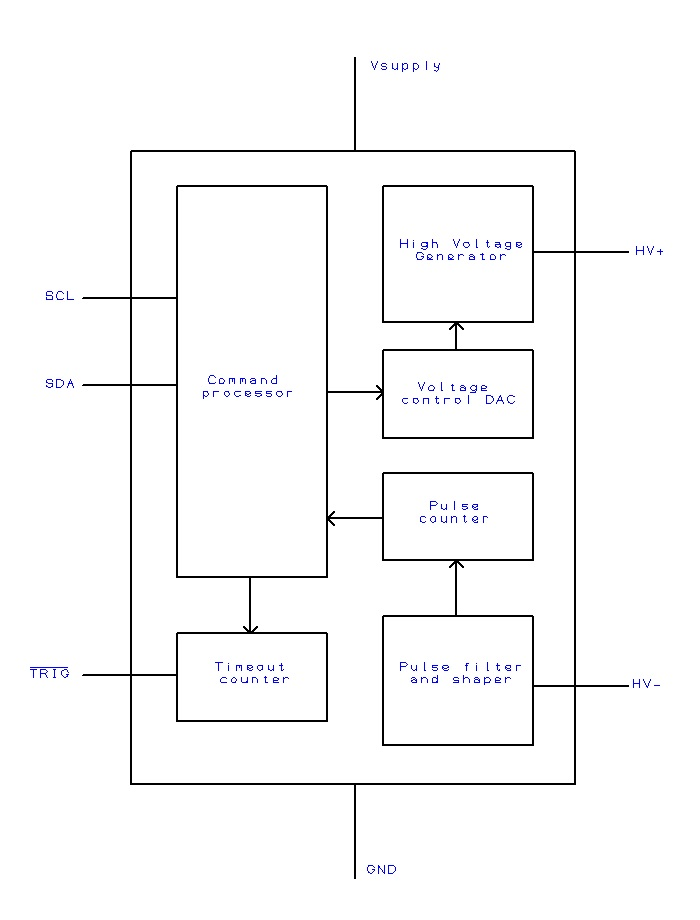
\includegraphics[width=3.2874in,height=4.3209in]{HVSUP01UM-img001.jpg} \stepcounter{Drawing}{\theDrawing}. Drawing:
Block diagram}
\end{minipage}
\end{center}
\subsection[]{\selectlanguage{english} }
\clearpage\subsection[Configuration]{\selectlanguage{english} Configuration}
\hypertarget{RefHeadingToc3521383566216}{}{\selectlanguage{english}
The device has two configurable parameters: the output voltage and the timeout.}

\subsubsection[Output voltage]{\selectlanguage{english} Output voltage}
\hypertarget{RefHeadingToc3541383566216}{}{\selectlanguage{english}
The voltage is a 16bits parameter with valid range from 400V to 600V. The given value is the output of the high voltage
front-end. Setting the voltage out of the allowed range will turn off the high voltage generator, while the rest of the
device, e.g. timeout and pulse counter, remains functional. }

{\selectlanguage{english}
The default value of the parameter is zero, i.e. the high voltage generator is turned off. For proper functionality the
value shall be configured to the operational voltage of the connected GM tube.}

\subsubsection[Timeout]{\selectlanguage{english} Timeout}
\hypertarget{RefHeadingToc3561383566216}{}{\selectlanguage{english}
The timeout is a 16 bits parameter in seconds. Setting the parameter to a value different than zero will generate an
active low signal on the TRIG pin of the device. Parameter zero will turn off the TRIG signaling. }

{\selectlanguage{english}
The default value of the parameter is zero. }

\subsection[Reading pulse count]{\selectlanguage{english} Reading pulse count}
\hypertarget{RefHeadingToc7033613373551}{}{\selectlanguage{english}
The pulse count value is a 24bits number. It is incremented by every pulse from the attached GM tube. The number of
pulses for a given radiation level is characteristic for each GM tube.}

{\selectlanguage{english}
If the timeout is set to zero then the counter value reflects the number of pulses since the last readout. If the
timeout is non-zero then the value is reflecting the number of pulses in the previous complete timeout period, and
remains the same until a new timeout occurs.}

\subsection[]{\selectlanguage{english} }
\clearpage\subsection[Reading factory data]{\selectlanguage{english} Reading factory data}
\hypertarget{RefHeadingToc7053613373551}{}\subsubsection[Firmware version]{\selectlanguage{english} Firmware version}
\hypertarget{RefHeadingToc7073613373551}{}{\selectlanguage{english}
The value is a 16 bits number, with MSB denoting the major and LSB denoting the minor software version.}

\subsubsection[Hardware version]{\selectlanguage{english} Hardware version}
\hypertarget{RefHeadingToc7093613373551}{}{\selectlanguage{english}
The value is a 16 bits number, with MSB denoting the major and LSB denoting the minor hardware version. }

\subsubsection[Serial number]{\selectlanguage{english} Serial number}
\hypertarget{RefHeadingToc7113613373551}{}{\selectlanguage{english}
The value is a 32 bits number that is unique for each device.}

\subsection[Typical operation]{\selectlanguage{english} Typical operation}
\hypertarget{RefHeadingToc2861383566216}{}{\selectlanguage{english}
The sensor can be connected to a 3V compliant I2C bus directly. The digital pins of the device are not 5V tolerant!}

{\selectlanguage{english}
Proper pull-up resistors shall be connected to the SCL and SDA lines, typically 4.7KOhm is sufficient. The open-drain
TRIG pin can be optionally connected to the wake-up, interrupt or reset pin of the MCU. This may be beneficial if the
host MCU is put in deep sleep mode between measurements. The HVSUP01 device can ensure that the host MCU is woken up
periodically by pulling down the TRIG pin for about 1ms, after the timeout elapses.}


\bigskip

\subsection[]{\selectlanguage{english} }
\clearpage\section[Digital interface]{\selectlanguage{english} Digital interface}
\hypertarget{RefHeadingToc1371383566216}{}\subsection[I2C (SCL and SDA)]{\selectlanguage{english} I2C (SCL and SDA)}
\hypertarget{RefHeadingToc1300441299070}{}{\selectlanguage{english}
The device can be interfaced to an I2C master host that supports Standard and Fast Mode communication. The sensor has a
set of registers that can be read and written. The registers can be accessed either individually or in group. The I2C
bus specification is not detailed here. For further reference see [1]}

{\selectlanguage{english}
The device can be accessed at the I2C address 0x6E. The address cannot be modified. }

{\selectlanguage{english}
The I2C command processor of the sensor evaluates the register changes after each STOP condition. Therefore it is
recommended to write the configuration parameters in atomic 16bits steps or consecutive registers in one 32bits step.}

{\selectlanguage{english}
\textit{Application hint: Although modifying individual register bytes is possible, it may lead to undesired
functionality. For example, if the timeout value 0x00FF is changed to 0x0101 in two steps then writing an individual
0x01 to LSB while the MSB is still 0x00, would trigger a wake-up request at the next second instead of 257 seconds.}}

\subsubsection[Access of the device]{\selectlanguage{english} Access of the device}
\hypertarget{RefHeadingToc12271084818799}{}{\selectlanguage{english}
The registers of the device appear like an array of bytes. The desired register can be selected by a one byte address
value that is written to the device. This may be followed by a sequence of write or read requests.}

\subsubsection[Writing data to the device]{\selectlanguage{english} Writing data to the device}
\hypertarget{RefHeadingToc12291084818799}{}{\selectlanguage{english}
Several consecutive bytes can be written with a single write sequence, followed by a STOP. The picture below
demonstrates and example, where two bytes are written to the register address 0x03 (timeout register).}



\begin{center}
\begin{minipage}{6.9252in}
{\selectlanguage{english}\itshape
 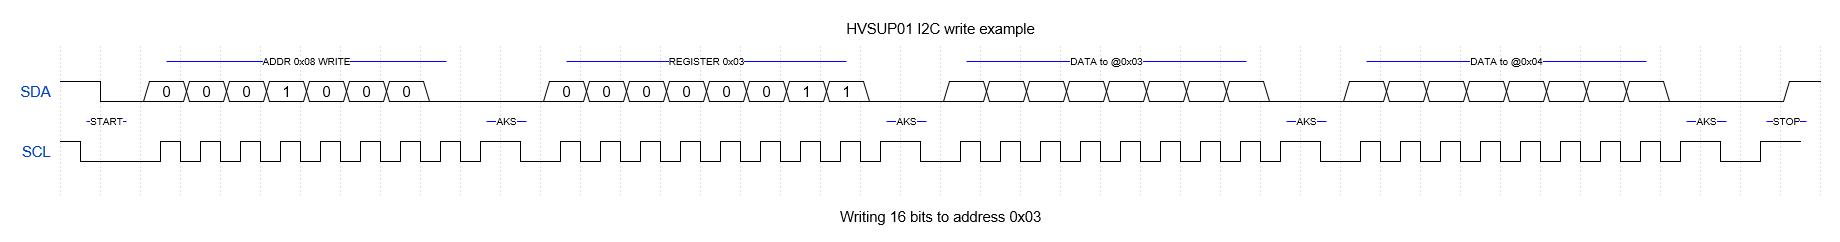
\includegraphics[width=6.9252in,height=0.9102in]{HVSUP01UM-img002.png} \stepcounter{Drawing}{\theDrawing}. Drawing: I2C
write}
\end{minipage}
\end{center}
\subsubsection[Reading data from the device]{\selectlanguage{english} Reading data from the device}
\hypertarget{RefHeadingToc12311084818799}{}{\selectlanguage{english}
\ Several consecutive bytes can be read then with a single read sequence that is terminated by a NACK from the host,
followed by a STOP sequence. The picture below demonstrates and example, where two bytes are read from the register
address 0x03 (timeout register).}



\begin{center}
\begin{minipage}{6.9252in}
{\selectlanguage{english}\itshape
 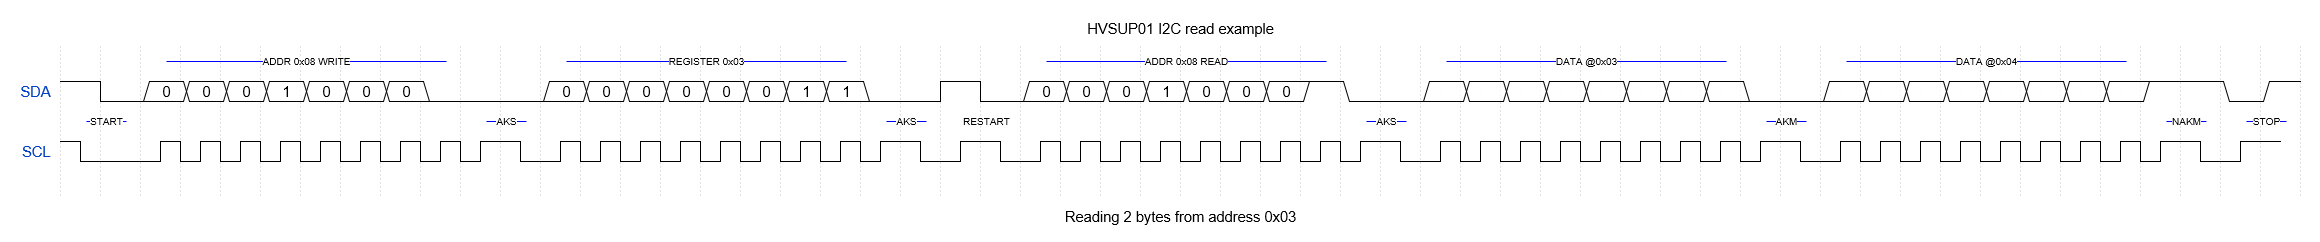
\includegraphics[width=6.9252in,height=0.722in]{HVSUP01UM-img003.png} \stepcounter{Drawing}{\theDrawing}. Drawing: I2C
read}
\end{minipage}
\end{center}
\subsubsection[Clock stretching]{\selectlanguage{english} Clock stretching}
\hypertarget{RefHeadingToc10431084818799}{}{\selectlanguage{english}
In order to maintain reliable communication in the specified I2C clock range, the device is using clock stretching. This
is completely transparent to the host application in most cases. If the host is using software emulation for I2C
communication, it might be necessary to set the clock stretch timeout explicitly. Observe the value specified in
chapter Timing parameters.}

\subsection[TRIG output]{\selectlanguage{english} TRIG output}
\hypertarget{RefHeadingToc1302441299070}{}{\selectlanguage{english}
The TRIG pin is a configurable open-drain output. The device is setting the pin to active LOW for 1 millisecond, with
the period that is defined by the timeout register value.}

\clearpage\section[Memory map]{\selectlanguage{english} Memory map}
\hypertarget{RefHeadingToc1391383566216}{}
\bigskip

\begin{flushleft}
\tablefirsthead{}
\tablehead{}
\tabletail{}
\tablelasttail{}
\begin{supertabular}{|m{0.7976598in}|m{1.9136599in}|m{1.3045598in}|m{1.1761599in}|}
\hline
{\selectlanguage{english}\bfseries Address} &
{\selectlanguage{english}\bfseries Register} &
{\selectlanguage{english}\bfseries Read/Write} &
{\selectlanguage{english}\bfseries Value after power-up}\\\hline
{\selectlanguage{english} 0x00} &
{\selectlanguage{english} PulseCount[7..0]} &
{\selectlanguage{english} Read only} &
{\selectlanguage{english} 0}\\\hline
{\selectlanguage{english} 0x01} &
{\selectlanguage{english} PulseCount[15..8]} &
{\selectlanguage{english} Read only} &
{\selectlanguage{english} 0}\\\hline
{\selectlanguage{english} 0x02} &
{\selectlanguage{english} PulseCount[23..16]} &
{\selectlanguage{english} Read only} &
{\selectlanguage{english} 0}\\\hline
{\selectlanguage{english} 0x03} &
{\selectlanguage{english} Timeout[7..0]} &
{\selectlanguage{english} Read - Write} &
{\selectlanguage{english} 0}\\\hline
{\selectlanguage{english} 0x04} &
{\selectlanguage{english} Timeout[15..8]} &
{\selectlanguage{english} Read - Write} &
{\selectlanguage{english} 0}\\\hline
{\selectlanguage{english} 0x05} &
{\selectlanguage{english} Voltage[7..0]} &
{\selectlanguage{english} Read - Write} &
{\selectlanguage{english} 0}\\\hline
{\selectlanguage{english} 0x06} &
{\selectlanguage{english} Voltage[15..8]} &
{\selectlanguage{english} Read - Write} &
{\selectlanguage{english} 0}\\\hline
{\selectlanguage{english} 0x07} &
{\selectlanguage{english} HW Version [7..0]} &
{\selectlanguage{english} Read only} &
{\selectlanguage{english} varies\footnotemark{}}\\\hline
{\selectlanguage{english} 0x08} &
{\selectlanguage{english} HW Version [15..8]} &
{\selectlanguage{english} Read only} &
{\selectlanguage{english} varies}\\\hline
{\selectlanguage{english} 0x09} &
{\selectlanguage{english} Firmware Version [7..0]} &
{\selectlanguage{english} Read only} &
{\selectlanguage{english} varies}\\\hline
{\selectlanguage{english} 0x0A} &
{\selectlanguage{english} Firmware Version [15..8]} &
{\selectlanguage{english} Read only} &
{\selectlanguage{english} varies}\\\hline
{\selectlanguage{english} 0x0B} &
{\selectlanguage{english} Serial Number[7..0]} &
{\selectlanguage{english} Read only} &
{\selectlanguage{english} varies}\\\hline
{\selectlanguage{english} 0x0C} &
{\selectlanguage{english} Serial Number[15..8]} &
{\selectlanguage{english} Read only} &
{\selectlanguage{english} varies}\\\hline
{\selectlanguage{english} 0x0D} &
{\selectlanguage{english} Serial Number[23..16]} &
{\selectlanguage{english} Read only} &
{\selectlanguage{english} varies}\\\hline
{\selectlanguage{english} 0x0E} &
{\selectlanguage{english} Serial Number[31..24]} &
{\selectlanguage{english} Read only} &
{\selectlanguage{english} varies}\\\hline
\end{supertabular}
\end{flushleft}
\footnotetext{The HW, Firmware and Serial number values designate a given device, hence there is no fix default value}

\bigskip

\subsection[Endianness]{\selectlanguage{english} Endianness}
\hypertarget{RefHeadingToc9151801770043}{}{\selectlanguage{english}
All register values are stored in little endian byte order.}

\clearpage\section[Connection setup]{Connection setup}
\hypertarget{RefHeadingToc13004280169782}{}A typical connection is demonstrated on picture \ref{seq:refDrawing3}\ below.


\subsubsection[]{}
\begin{center}
\begin{minipage}{6.9252in}
{\selectlanguage{english}\itshape
 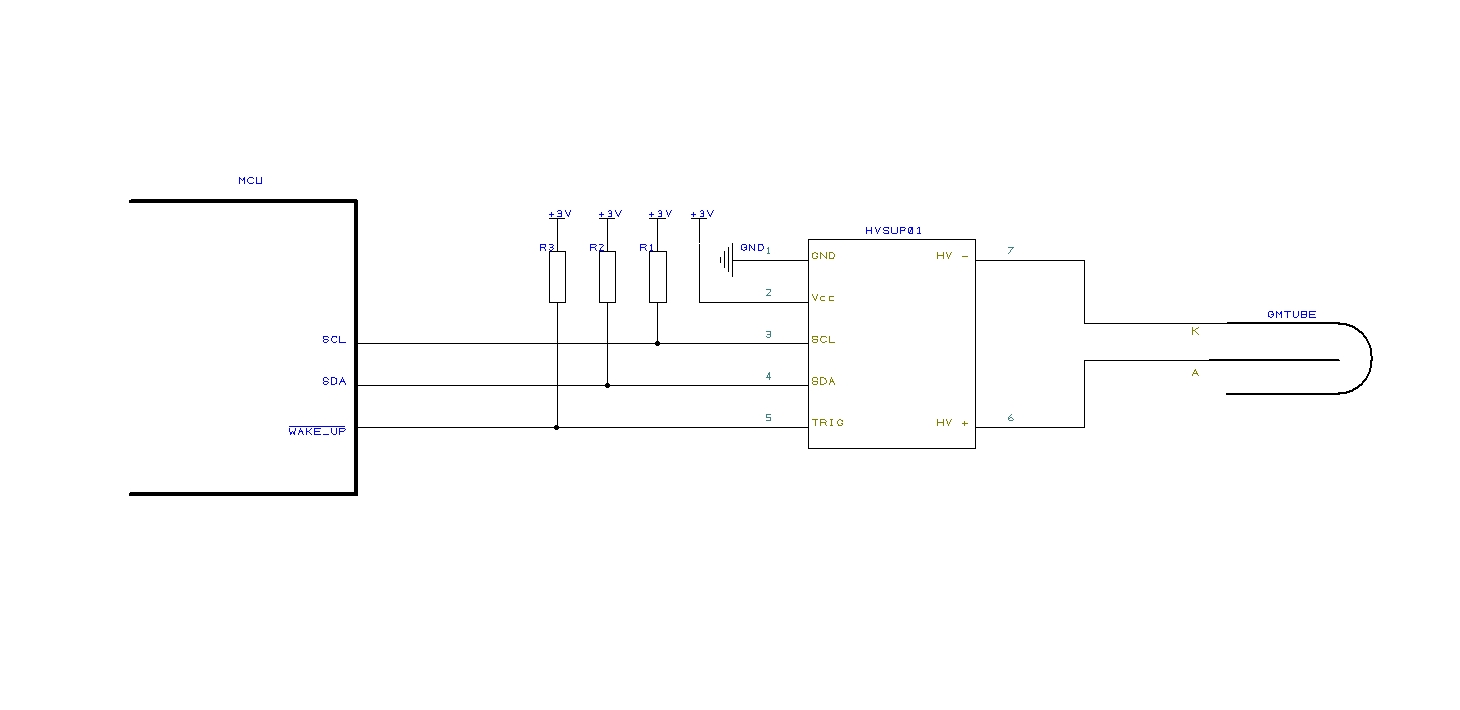
\includegraphics[width=6.6953in,height=2.1382in]{HVSUP01UM-img004.jpg} \newline
{\refstepcounter{Drawing}\theDrawing\label{seq:refDrawing3}}. Drawing: Typical connection}
\end{minipage}
\end{center}
\subsubsection{Power supply}
\hypertarget{RefHeadingToc13044280169782}{}During normal operation the sensor is generating very short, high current
pulses on the power input. If the circuit is powered from a low power LDO rated less than 400mA, then it is suggested
to connect a relatively large capacitor (e.g. 0.3F supercap) between Vcc and GND and connect a series resistor in a few
Ohms range between the LDO and the capacitor. See picture \ref{seq:refDrawing4}\ below.



\begin{center}
\begin{minipage}{6.6953in}
{\itshape
 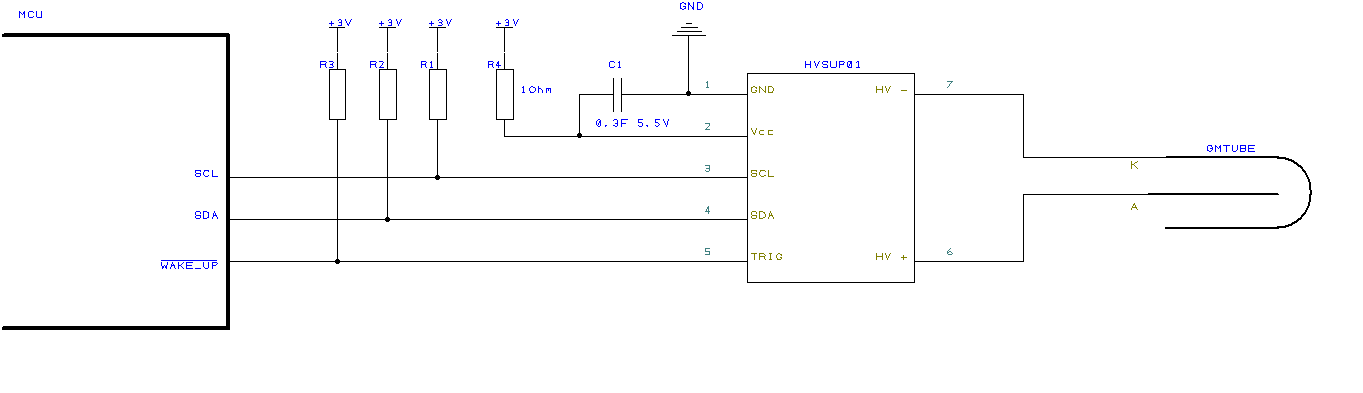
\includegraphics[width=6.6953in,height=1.6898in]{HVSUP01UM-img005.png}
{\refstepcounter{Drawing}\theDrawing\label{seq:refDrawing4}}. Drawing: Typical connection with weak power supply}
\end{minipage}
\end{center}
\subsubsection[Detector noise]{\selectlanguage{english} Detector noise}
\hypertarget{RefHeadingToc4061383566216}{}The High Voltage front-end contains filtering and signal shaping features to
eliminate most electrical noise that could influence the measurement. Large noise signal on the terminals of the sensor
can still negatively affect the pulse count value. Therefore it is recommended to ensure that the connection between
the device and the detector tube is as short as possible. If the distance between the sensor and the tube is longer
than 15-30cm then shielded cable can be used with two inner conductors.

\clearpage\section[Package]{\selectlanguage{english} Package}
\hypertarget{RefHeadingToc1411383566216}{}{\selectlanguage{english}
The sensor is available in epoxy filled ABS package.}

\subsection[Pin configuration]{\selectlanguage{english} Pin configuration}
\hypertarget{RefHeadingToc1431383566216}{}{\selectlanguage{english}
Bottom view of the device with pin numbers:}



\begin{center}
\begin{minipage}{2.0272in}
{\selectlanguage{english}\itshape
[Warning: Draw object ignored]\stepcounter{Drawing}{\theDrawing}. Drawing: Pin numbering}
\end{minipage}
\end{center}
\begin{flushleft}
\tablefirsthead{}
\tablehead{}
\tabletail{}
\tablelasttail{}
\begin{supertabular}{|m{1.1712599in}|m{3.2962599in}|}
\hline
{\selectlanguage{english}\bfseries Pin number} &
{\selectlanguage{english}\bfseries Pin function}\\\hline
{\selectlanguage{english} 1} &
{\selectlanguage{english} GND}\\\hline
{\selectlanguage{english} 2} &
{\selectlanguage{english} Vcc}\\\hline
{\selectlanguage{english} 3} &
{\selectlanguage{english} SCL}\\\hline
{\selectlanguage{english} 4} &
{\selectlanguage{english} SDA}\\\hline
{\selectlanguage{english} 5} &
{\selectlanguage{english} TRIG}\\\hline
{\selectlanguage{english} 6} &
{\selectlanguage{english} HV +}\\\hline
{\selectlanguage{english} 7} &
{\selectlanguage{english} HV -}\\\hline
\end{supertabular}
\end{flushleft}
\subsection[]{\selectlanguage{english} }
\clearpage\subsection[Outline dimensions]{\selectlanguage{english} Outline dimensions}
\hypertarget{RefHeadingToc1451383566216}{}{\selectlanguage{english}
All dimensions are in millimeters.}

\begin{flushleft}
\tablefirsthead{}
\tablehead{}
\tabletail{}
\tablelasttail{}
\begin{supertabular}{|m{2.23236in}|m{2.0462599in}|}
\hline
{\selectlanguage{english} Length x width} &
{\selectlanguage{english} 36 mm x 36 mm}\\\hline
{\selectlanguage{english} Height without pins} &
{\selectlanguage{english} 15 mm}\\\hline
{\selectlanguage{english} Height with pins} &
{\selectlanguage{english} 21.5 mm}\\\hline
{\selectlanguage{english} Pin width} &
{\selectlanguage{english} 0.64 mm x 0.64 mm}\\\hline
\end{supertabular}
\end{flushleft}

\bigskip

\subsection[Pin placement dimensions]{\selectlanguage{english} Pin placement dimensions}
\hypertarget{RefHeadingToc12331084818799}{}
\bigskip



\begin{center}
\begin{minipage}{3.2563in}
{\selectlanguage{english}\itshape
 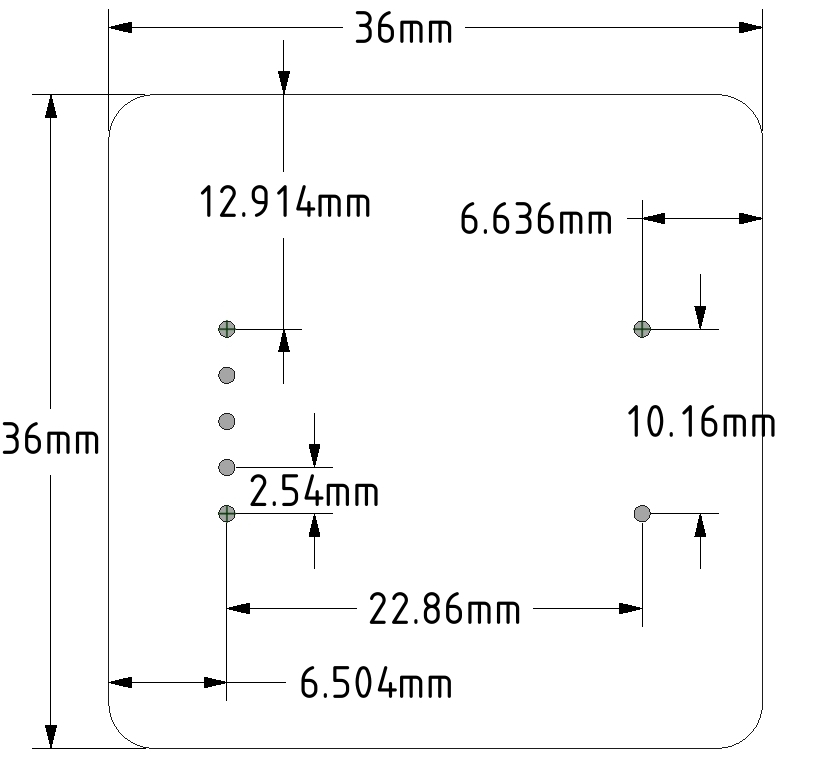
\includegraphics[width=3.2016in,height=2.9811in]{HVSUP01UM-img006.jpg} \stepcounter{Drawing}{\theDrawing}. Drawing:
Mechanical drawing}
\end{minipage}
\end{center}
\clearpage
\bigskip

\subsection[Soldering and assembly recommendations]{\selectlanguage{english} Soldering and assembly recommendations}
\hypertarget{RefHeadingToc1471383566216}{}{\selectlanguage{english}
The HVSUP01 sensor is primarily suitable for manual soldering. The pins are gold plated which provides excellent
electrical connection when used with solder-less breadboards, too.}

{\selectlanguage{english}
The device is not suitable for any assembly process that could expose the encapsulation to temperatures higher than 80
{\textdegree}C or 176 {\textdegree}F.}

\clearpage\section[References]{\selectlanguage{english} References}
\hypertarget{RefHeadingToc9651801770043}{}\begin{flushleft}
\tablefirsthead{}
\tablehead{}
\tabletail{}
\tablelasttail{}
\begin{supertabular}{|m{0.7330598in}|m{6.03236in}|}
\hline
\liststyleLii
\begin{enumerate}
\item ~

\end{enumerate}
 &
{\selectlanguage{english} \href{https://www.nxp.com/docs/en/user-guide/UM10204.pdf}{\foreignlanguage{english}{I2C-bus
specification and user manual}}}\\\hline
~
 &
~
\\\hline
~
 &
~
\\\hline
\end{supertabular}
\end{flushleft}
\section[]{\selectlanguage{english} }
\clearpage\section[Legal disclaimer]{\selectlanguage{english} Legal disclaimer}
\hypertarget{RefHeadingToc1811383566216}{}{\selectlanguage{english}
The HVSUP01 sensor is intended for educational purpose only. }

{\selectlanguage{english}
The sensor may not fit for use in environment and purpose where the malfunction of the device could lead to bodily harm
or property damage. }

{\selectlanguage{english}
The user of the device understands and agrees that the prototyping sensor has not been fully certified, therefore its output data
must not be used for quantitative judgment of potentially high radiation. }

{\selectlanguage{english}
It is the user's responsibility to determine whether the product fits for the intended use in the prototyping
environment.}

{\selectlanguage{english}
The author of this project shall not be liable to any damages related to use of the device.}

{\selectlanguage{english}
{The sensor is not a Finished Appliance. In case the equipment is used as part of a Finished Appliance then the user of the device must take
responsibility for galvanic insulation from the environment and to follow regulatory guidelines, for example CE marking.}

\subsection[RoHS compliance]{\selectlanguage{english} RoHS compliance}
\hypertarget{RefHeadingToc3581383566216}{}{\selectlanguage{english}
Although the device has been built from RoHS compliant parts with RoHS compliant assembly process, no formal statement
is given here about RoHS compliance.}
\end{document}
